\chapter{Remaining Useful Life Prediction}
\label{chap: rul}

In this chapter, we propose a framework for predicting RUL of EoL products based on the ultrasonic testing. The framework has two parts: \begin{enumerate*}[label=\itshape\alph*\upshape)]
    \item a ML classification task and
    \item a RUL inference procedure based on a S-N curve.
\end{enumerate*}  First, ultrasonic signals are fed into ML classifiers to predict the loading condition and the number of fatigue cycles that a sample has gone through. Second, we estimate RUL from a S-N curve with the predicted loading condition and fatigue cycles.

\section{Problem formulation}
\label{sec: rul prob formulation}
Given the goal of predicting the RUL of EoL products, we need to formulate this as a ML problem first. In this section, We discuss possible formulations by considering the characteristics of the fatigue dataset and the impact on the ML system in practice.

\subsection{Dataset}
In this RUL prediction task, the dataset is constructed on the ultrasonic measurements on the interrupted fatigue testing specimens in Table \ref{table: interrupted specimens}. There are 15 specimens and each of these were measured at 9 locations alongside 3 repeated measurements, producing 405 observations in total. Notice that we treat one measurement location in one specimen as a sample in the model training and validation procedure with LOGOCV, as described in Section \ref{sec: model train and val}. Besides, each specimen is tested by a combination from 4 loading amplitudes and 3 fatigue levels (the percentage of fatigue life), which forms the labels of a specimen.

\subsection{Target variables}
Obviously, RUL is directly translated by the percentage of fatigue life that a sample has gone through. The percentage of fatigue life as a continuous target variable is normally treated as a regression task. However, since we only have 3 different percentage of fatigue life in the dataset, which is not ideal for regression modeling, we decided to view the percentage of fatigue life as a discrete variable and the problem becomes a classification task.

Loading amplitude is another target variable to be considered because loading condition affects the mechanism of fatigue damage in a material. For instance, at 33\% fatigue life, a sample undergoes 11.7 kN loading and a sample undergoes 14.7 kN loading could exist different fatigue damages. Hence, we place a label that is a combination of loading amplitude and the percentage of fatigue life on each sample. Table \ref{table: rul dataset} presents the labeled RUL prediction dataset.

\begin{table}[tb]
    \centering
    \caption{Summary of the RUL prediction dataset}
    \label{table: rul dataset}
    \begin{tabularx}{\textwidth}{
      >{\centering\arraybackslash\hsize=0.5\hsize}X|
      >{\centering\arraybackslash\hsize=0.6\hsize}X|
      >{\centering\arraybackslash\hsize=0.6\hsize}X|
      >{\centering\arraybackslash}X
    }\hline
      Specimen ID & Measurement Locations & Number of Repeated Measurements & Label (amplitude, percent of fatigue life) \\
      \hline
          1&\multirow{15}{*}{$1\sim 9$}&\multirow{15}{*}{3}&\multirow{2}{*}{Class 1 (11.7 kN, 33\%)}\\
          2& & & \\
          \cline{1-1}\cline{4-4}
          3& & &\multirow{2}{*}{Class 2 (11.7 kN, 67\%)}\\
          4& & & \\
          \cline{1-1}\cline{4-4}
          5& & &\multirow{2}{*}{Class 3 (12.7 kN, 33\%)}\\
          6& & & \\
          \cline{1-1}\cline{4-4}
          7& & &\multirow{2}{*}{Class 4 (12.7 kN, 67\%)}\\
          8& & & \\
          \cline{1-1}\cline{4-4}
          9& & &\multirow{2}{*}{Class 5 (14.7 kN, 33\%)}\\
          10& & & \\
          \cline{1-1}\cline{4-4}
          11& & &\multirow{2}{*}{Class 6 (14.7 kN, 67\%)}\\
          12& & & \\
          \cline{1-1}\cline{4-4}
          13& & &\multirow{3}{*}{Class 0 (0 kN, 0\%)}\\
          14& & & \\
          15& & & \\\hline
    \end{tabularx}
\end{table}

\section{Design of classifiers}
\label{sec: design of classifiers}
In this section, classifiers are designed for predicting the loading condition (amplitude) and the percent of fatigue life that a sample had experienced. Several classifiers are developed and the performance of each of those methods is evaluated based on the model development procedure in Chapter \ref{chap: model}.

\subsection{Multi-class classifier}
A multi-class classifier is trained to classify a sample into one of the 7 classes. Figure XXX shows the inference process of a multi-class classifier. In multi-class problems, the classes are mutually exclusive. For example, class 1 and class 3 have nothing related. Despite we claimed that various loading conditions result in different fatigue behaviors in material, however, some similarities are still existed, e.g., at 33\% fatigue life, samples undergone 11.7 kN and 12.7 kN are expected to be on a similar damage level. This idea can be applied to the commonality in samples at different percents of fatigue life as well. With the assumption about mutual exclusivity, multi-class formulation does not capture these characteristics of the data.

\subsection{Multi-output classifier}
\label{subsec: multi-output classifier}
On the other hand, multi-output classification is capable of dealing with mutually non-exclusive classes by predicting the loading amplitude and percentage of fatigue life separately. A multi-output classier outputs multiple labels, where each label is considered a multi-class classification problem. In this design, we build one classifier for predicting the loading amplitude from input signals; another one for classifying a signal into one of the percentages of fatigue life. Then, the two predicted labels are combined based on a rule-based algorithm to output a class label that is consistent with the label in the dataset, as depicted in Figure XXX. We call these two classifiers loading amplitude classifier (LAC) and fatigue cycle classifier (FCC), respectively. Each of the two classifiers are trained separately with the same model development procedure but different target variables. As a result, unlike the single multi-class classifier trying to learn a way to separate 7 classes, the multi-output classification builds LAC for a 4-class problem for loading amplitude and FCC for a 3-class problem for the percentage of fatigue life, which makes the problems easier to learn.

\subsection{Two-stage classifier}
Table XXX shows the design of a two-stage classifier. Extended from the idea of multi-output classifier in Subsection \ref{subsec: multi-output classifier}, a two-stage classifier is a classifier chains which predicts the loading amplitude and percentage of fatigue life in an order. The classification starts with a LAC and the predicted loading amplitude is added to the feature space of a \fcctwo. By utilizing the predicted label as a feature for next classifiers, the label dependence is preserved, i.e., the prediction of the percentage of fatigue life sample has undergone is associated with its loading amplitude. In this case, we put the LAC before the \fcctwo \  because sometimes the loading condition is given in real life scenarios. Note that, in the training phase, the true loading amplitude is used to train the \fcctwo, but the \fcctwo \ takes the predicted loading amplitude as one of the input features to do inference.

\subsection{Hierarchical classifier}
We further transform the multi-output task into a hierarchical classification scheme which is composed of multiple local classifiers based on a tree structure, shown in Figure XXX. One advantage of the hierarchical classification is to exploit parent-child class relationships present in the class hierarchy. Here, we train local classifiers per parent node in the taxonomy of the hierarchical classification problem. Specifically, one LAC and three FCCs for each loading amplitude are built, where each of the FCCs are trained by samples with the corresponding loading amplitude only. A prediction is inferred by the following manner: 
\begin{enumerate*}[label=\itshape\alph*\upshape)]
    \item the LAC first output the loading amplitude for input LU and NLU signals.
    \item the predicted loading amplitude is also used to choose one of the FCCs for predicting the percentage of fatigue life.
    \item the FCC predicts the percentage of fatigue life.
\end{enumerate*}
For example, 11.7 kN loading amplitude is predicted by the LAC. Therefore, FCC\textsubscript{11.7 kN} where the subscript stands for the loading amplitude that the classier corresponds to, is selected and outputs a 33\% fatigue life prediction. Finally, the predicted result is Class 1 (11.7 kN, 33\%).

\subsection{Evaluation metrics}
We calculate accuracy, recall, precision, and F1-measure to evaluate a classifier's performance with the LOGOCV result, and confusion matrices are also presented. Although there exist other evaluation metrics for multi-output problems, we evaluate the aforementioned classifiers in a unified multi-class classification problem with the label defined in Table \ref{table: rul dataset}. Thus, these classifiers are comparable with each other. Since there is not much class imbalance in the dataset, accuracy is an overall indicator for a model's performance. Furthermore, the model's performance on each class is provided by recall, precision and F1-measure. Finally, confusion matrices serve as a visualization for summarizing the detailed result of the testing of a classifier. We let practitioners to decide the importance of each metric as it depends on different scenarios. For example, recall may be more important than precision in classifying highly-fatigued samples due to the consideration of safety.

\subsection{Results}
This subsection summarizes the results of the developed classifier designs. Table \ref{table: summary class algo} presents the learning algorithms and the number of features determined by the model development procedure in Section \ref{chap: model}. Figure \ref{fig: f1 comparison} depicts the performance of each classifier design by class. Overall, it is noticed that the proposed hierarchical classifier outperforms the other methods discussed in Section \ref{sec: design of classifiers} for every class except Class 6.Therefore, the hierarchical classifier is chosen to demonstrate the RUL estimation algorithm in the following sections.

The recall, precision, and F1-score for the hierarchical classifier is illustrated in Fig

\begin{table}[tb]
    \centering
    \caption{Summary of classification algorithms and model performance}
    \label{table: summary class algo}
    \begin{tabularx}{\textwidth}{
      >{\centering\arraybackslash}X
      >{\centering\arraybackslash}X
      >{\centering\arraybackslash}X
      >{\centering\arraybackslash}X
    }
    \toprule
      Design of Classifiers & Algorithm & No. Selected Features & Macro Average F1-score \\
      \midrule
      \multirow{4}{*}{Multi-class} & & \multirow{4}{*}{35} & \multirow{4}{*}{0.75} \\
      & Logistic & & \\
      & regression & & \\
      & & & \\
      % 
      \multirow{4}{*}{Multi-output} & & & \multirow{4}{*}{0.77} \\
      & Logistic & 59 (LAC) & \\
      & regression & 51 (FCC) & \\ 
      & & & \\
      %
      \multirow{4}{*}{Two-stage} & & & \multirow{4}{*}{0.80} \\
      & Logistic & 59 (LAC) & \\
      & regression & 51 (FCC\textsubscript{two-stage}) & \\
      & & & \\
      %
      \multirow{4}{*}{Hierarchical} &  & 59 (LAC) & \multirow{4}{*}{0.83} \\
      & Logistic & 10 (FCC\textsubscript{11.7 kN}) & \\
      & regression & 40 (FCC\textsubscript{12.7 kN}) & \\
      &  & 6 (FCC\textsubscript{14.7 kN}) & \\
      %
      \bottomrule
    \end{tabularx}
\end{table}

\begin{figure}[tb]
    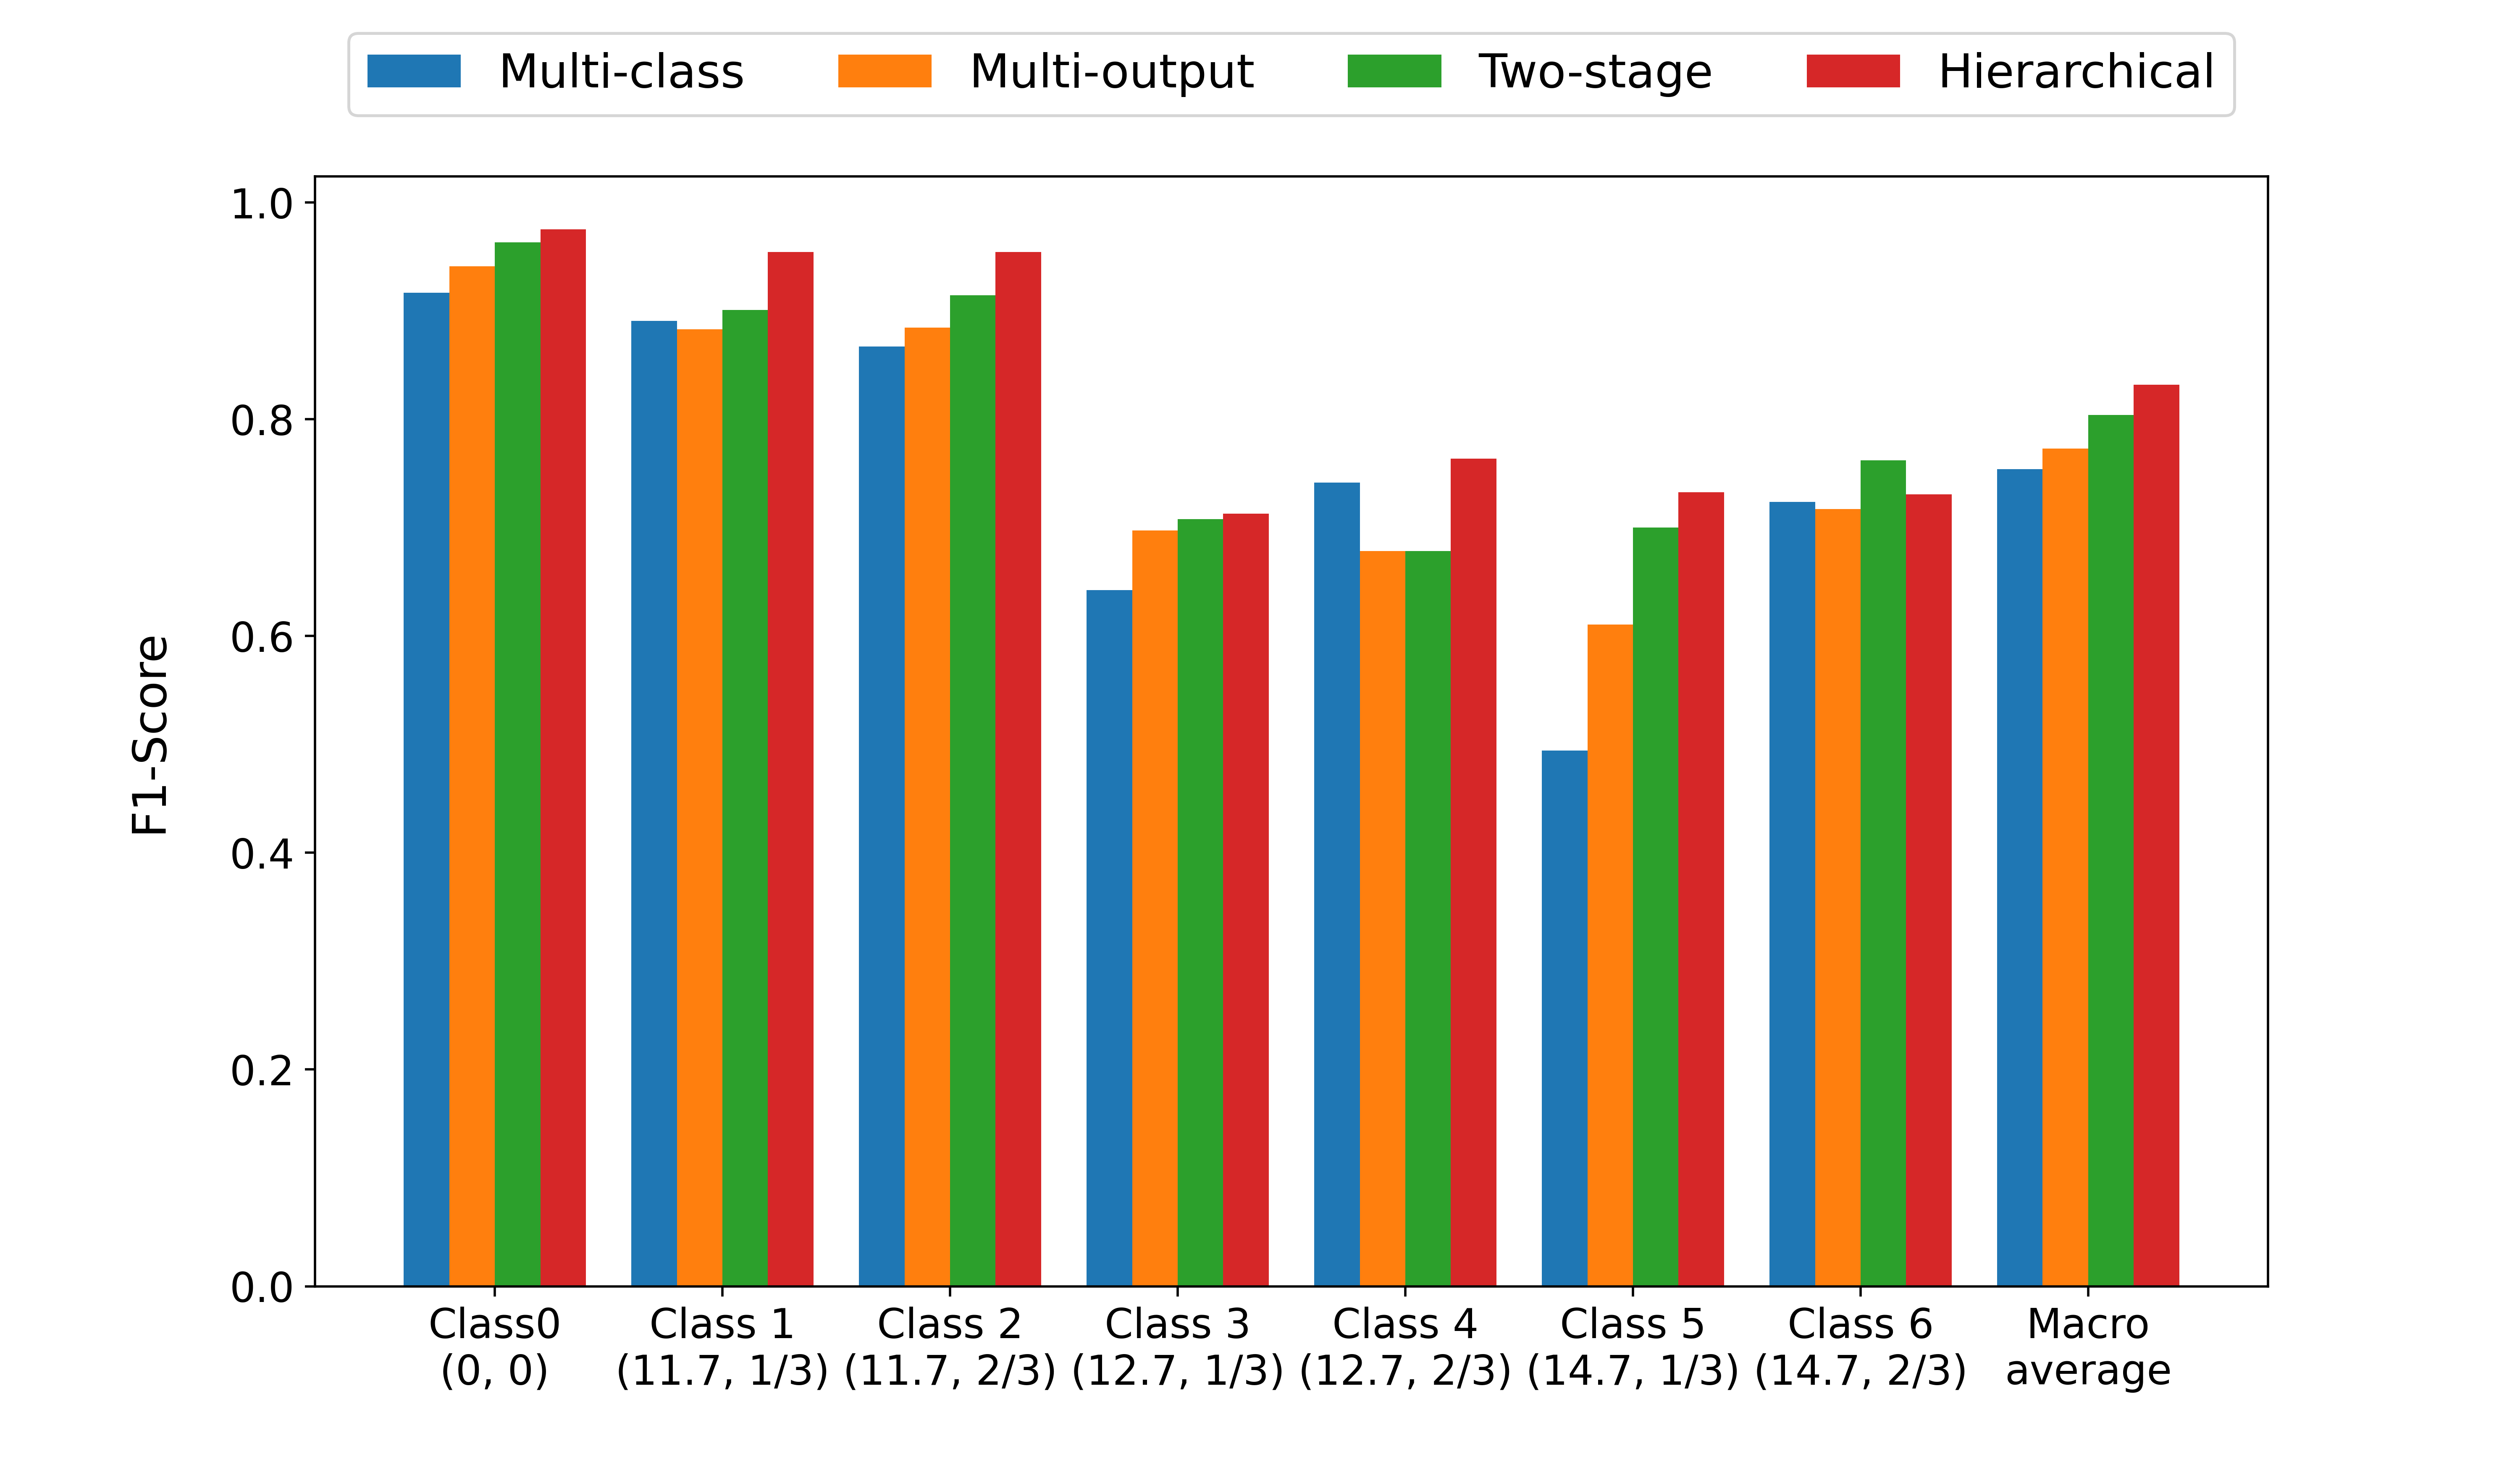
\includegraphics[width=\linewidth]{fig/f1_comparison.png}
    \caption{Comparison of F1-score by class and classifier designs}
    \label{fig: f1 comparison}
\end{figure}

% \begin{figure}
%     \includegraphics[width=\linewidth]{fig/}
% \end{figure}


\section{RUL estimation with a S-N curve}
In the proposed framework, after obtaining the predicted loading amplitude and percentage of fatigue life, we estimate the RUL for a sample with the S-N curve of that material.

\subsection{S-N curve with statistical distributions}
Although a S-N curve is often referred to the best-fit line for fatigue data, fatigue life data can be modeled as statistical distributions to account for the variability in fatigue life. The randomness in the fatigue life comes from the stochastic behavior in fatigue process and the variance of microstructure in materials. As a result, the fatigue life has been widely modeled by statistical distributions including Gaussian (normal), log-normal, and Weibull distribution. Due to the limited amount of available fatigue life data in this research, we use a Gaussian normal distribution to model the fatigue life $X_a$ at a loading amplitude $a$ as
\begin{equation}
    X_a \sim Normal(\bar{x_a}, \frac{s_a^2}{n_a})
\end{equation}
where $\bar{x_a}$ is the sample mean, $s_a$ is the sample standard variance, and $n_a$ is the sample size of fatigue data at loading amplitude $a$.

\subsection{RUL inference procedure}
A S-N curve serves as a look-up table for linking the classifier's predictions to the RUL. The inference procedure is detailed below:
\begin{enumerate}
    \item Plotting the predicted loading amplitude and percentage of fatigue life. For example, the prediction, Class 1 (11.7 kN, 33\% fatigue life), is plotted as the red dot in Figure XXX.
    \item Determine the fatigue life with the corresponding loading amplitude from the S-N curve. The fatigue life can be in the format of a single value such as the median fatigue life or a statistical distribution.
    \item If the fatigue life is represented by a value, the RUL can be estimated by Equation \eqref{eq: rul - value}: 
    \begin{equation}
        \label{eq: rul - value}
        RUL = N_{fl} - N_{c}
    \end{equation}
    where $N_{fl}$ is the fatigue life from a S-N curve and $N_c$ is the number of cycles translated from the predicted percentage of fatigue life a sample has undergone.

    If the fatigue life at a given loading amplitude is modeled as a normal distribution, one way to estimate the RUL of a sample is to transform the fatigue life distribution by a factor of the predicted percentage of fatigue life, as in Equation \eqref{eq: fatigue life dist} to \eqref{eq: rul - dist}:
    \begin{equation}
        \label{eq: fatigue life dist}
        X \sim Normal(\mu, \sigma^2)
    \end{equation}
    \begin{equation}
        \label{eq: rul transform}
        Y = pX
    \end{equation}
    \begin{equation}
        \label{eq: rul - dist}
        Y \sim Normal(p\mu, p^2\sigma^2)
    \end{equation}
    where $Y$ is a random variable representing the RUL of a sample; $X$ follows a normal distribution $Normal (\mu, \sigma^2)$ with $\mu$ as the mean and $\sigma^2$ as the variance of the fatigue life, and $F$ is scaled by $p$ which is the predicted percentage of fatigue life. Then, the point estimates, e.g., mean, median, or 25\% quantile, as well as the interval estimate of RUL can be inferred. For instance, the 90\% confidence interval of RUL is
    \begin{equation}
        CI = [\mu - z_{0.05} p \sigma,\ \mu + z_{0.95} p \sigma]
    \end{equation}
\end{enumerate}

\subsection{Examples}
In this subsection, we demonstrate two examples of the RUL estimation based on the proposed framework. Because the true fatigue life of the testing samples in the interrupted fatigue testing data is not available, we do not evaluate the accuracy quantitatively in this stage. Instead, the estimated 90\% confidence intervals of the RUL for specimen A and B are presented in Table X and X.

\section{Discussion}
One advantage of using the S-N curve to estimate RUL is that it can be quickly adopted to those materials whose S-N curve has constructed, which is common in the industry.